\section{ASR Specialization}
\label{sec:asr}

% \subsection{Why ASR is an Ideal Setting for Verifiable Multi-Token Decoding}
% The ASR branch of StepAudio 2.5 makes a strong systems claim: 
% ASR is a particularly favorable domain for multi-token prediction~\citep{leviathan2023fast,chen2023accelerating,cai2024medusa,gloeckle2024betterfaster,zhang2025mamba}. Unlike open-ended generation, where future tokens often branch semantically, speech recognition is acoustically constrained: given the audio and a correct prefix, the next tokens follow deterministically. Leveraging this, the model adds future-token branches, proposes multiple tokens per step, and accepts only the verified prefix. Incorrect proposals simply shorten the accepted lookahead without corrupting the final output. Thus, the verification rule makes acceleration compatible with reliability.


% ASR is a particularly favorable domain for multi-token prediction~\citep{leviathan2023fast,chen2023accelerating,cai2024medusa,gloeckle2024betterfaster,zhang2025mamba}. In open-ended text generation, future tokens often branch semantically, so long speculative prefixes can be fragile. In speech transcription, by contrast, the local future is heavily constrained by the acoustic signal. Given the audio and the accepted transcript prefix, the next few tokens are usually not a matter of stylistic freedom but of faithful continuation.

% This observation leads to the central ASR innovation. Rather than viewing multi-token prediction as a generic decoding trick, the ASR branch turns it into a task-aligned primitive. The model attaches multiple future-token branches to the decoder, proposes several transcript tokens in one forward step, and accepts only the verified prefix. Incorrect proposals do not corrupt the final transcript; they merely shorten the accepted lookahead. The verification rule therefore makes acceleration compatible with reliability.

% \subsection{ASR Architecture and MTP Design}

% StepAudio 2.5 ASR remains intentionally conservative in the backbone but aggressive in its decoding path. The architecture follows the StepAudio encoder-adapter-decoder pattern, augmented with an \mtpmodel\ head that proposes verifiable future transcript tokens, as shown in Figure~\ref{fig:asr_architecture}. This design is organized around three goals: strong recognition accuracy from a large decoder, efficient serving through multi-token proposals, and native long-form transcription through a 32K context window.

StepAudio 2.5 ASR follows the StepAudio encoder-adapter-decoder pattern, augmented with an \mtpmodel\ head that proposes verifiable future transcript tokens, as shown in Figure~\ref{fig:asr_architecture}. %This design is organized around three goals: strong recognition accuracy from a large decoder, efficient serving through multi-token proposals, and native long-form transcription through a 32K context window.
% \textbf{MTP as verifiable lookahead.} 
At decoding position $t$, the main branch predicts the next transcript token $x_{t+1}$. The $h$-th MTP branch predicts $x_{t+1+h}$ for $h\in\{1,\ldots,5\}$, so one forward step produces a six-token proposal. During inference, the proposal is accepted only as a verified prefix: once a future token disagrees with the normal decoding path, later proposed tokens are rejected and decoding continues autoregressively from the accepted prefix. This verification mechanism ensures that MTP acts strictly as an acceleration primitive. % It improves serving efficiency by increasing the tokens emitted per step, while maintaining the safety rule that determines the final transcript.
\begin{figure}[tbp]
\centering
% \includegraphics[width=\linewidth]{figures/architecture.pdf}
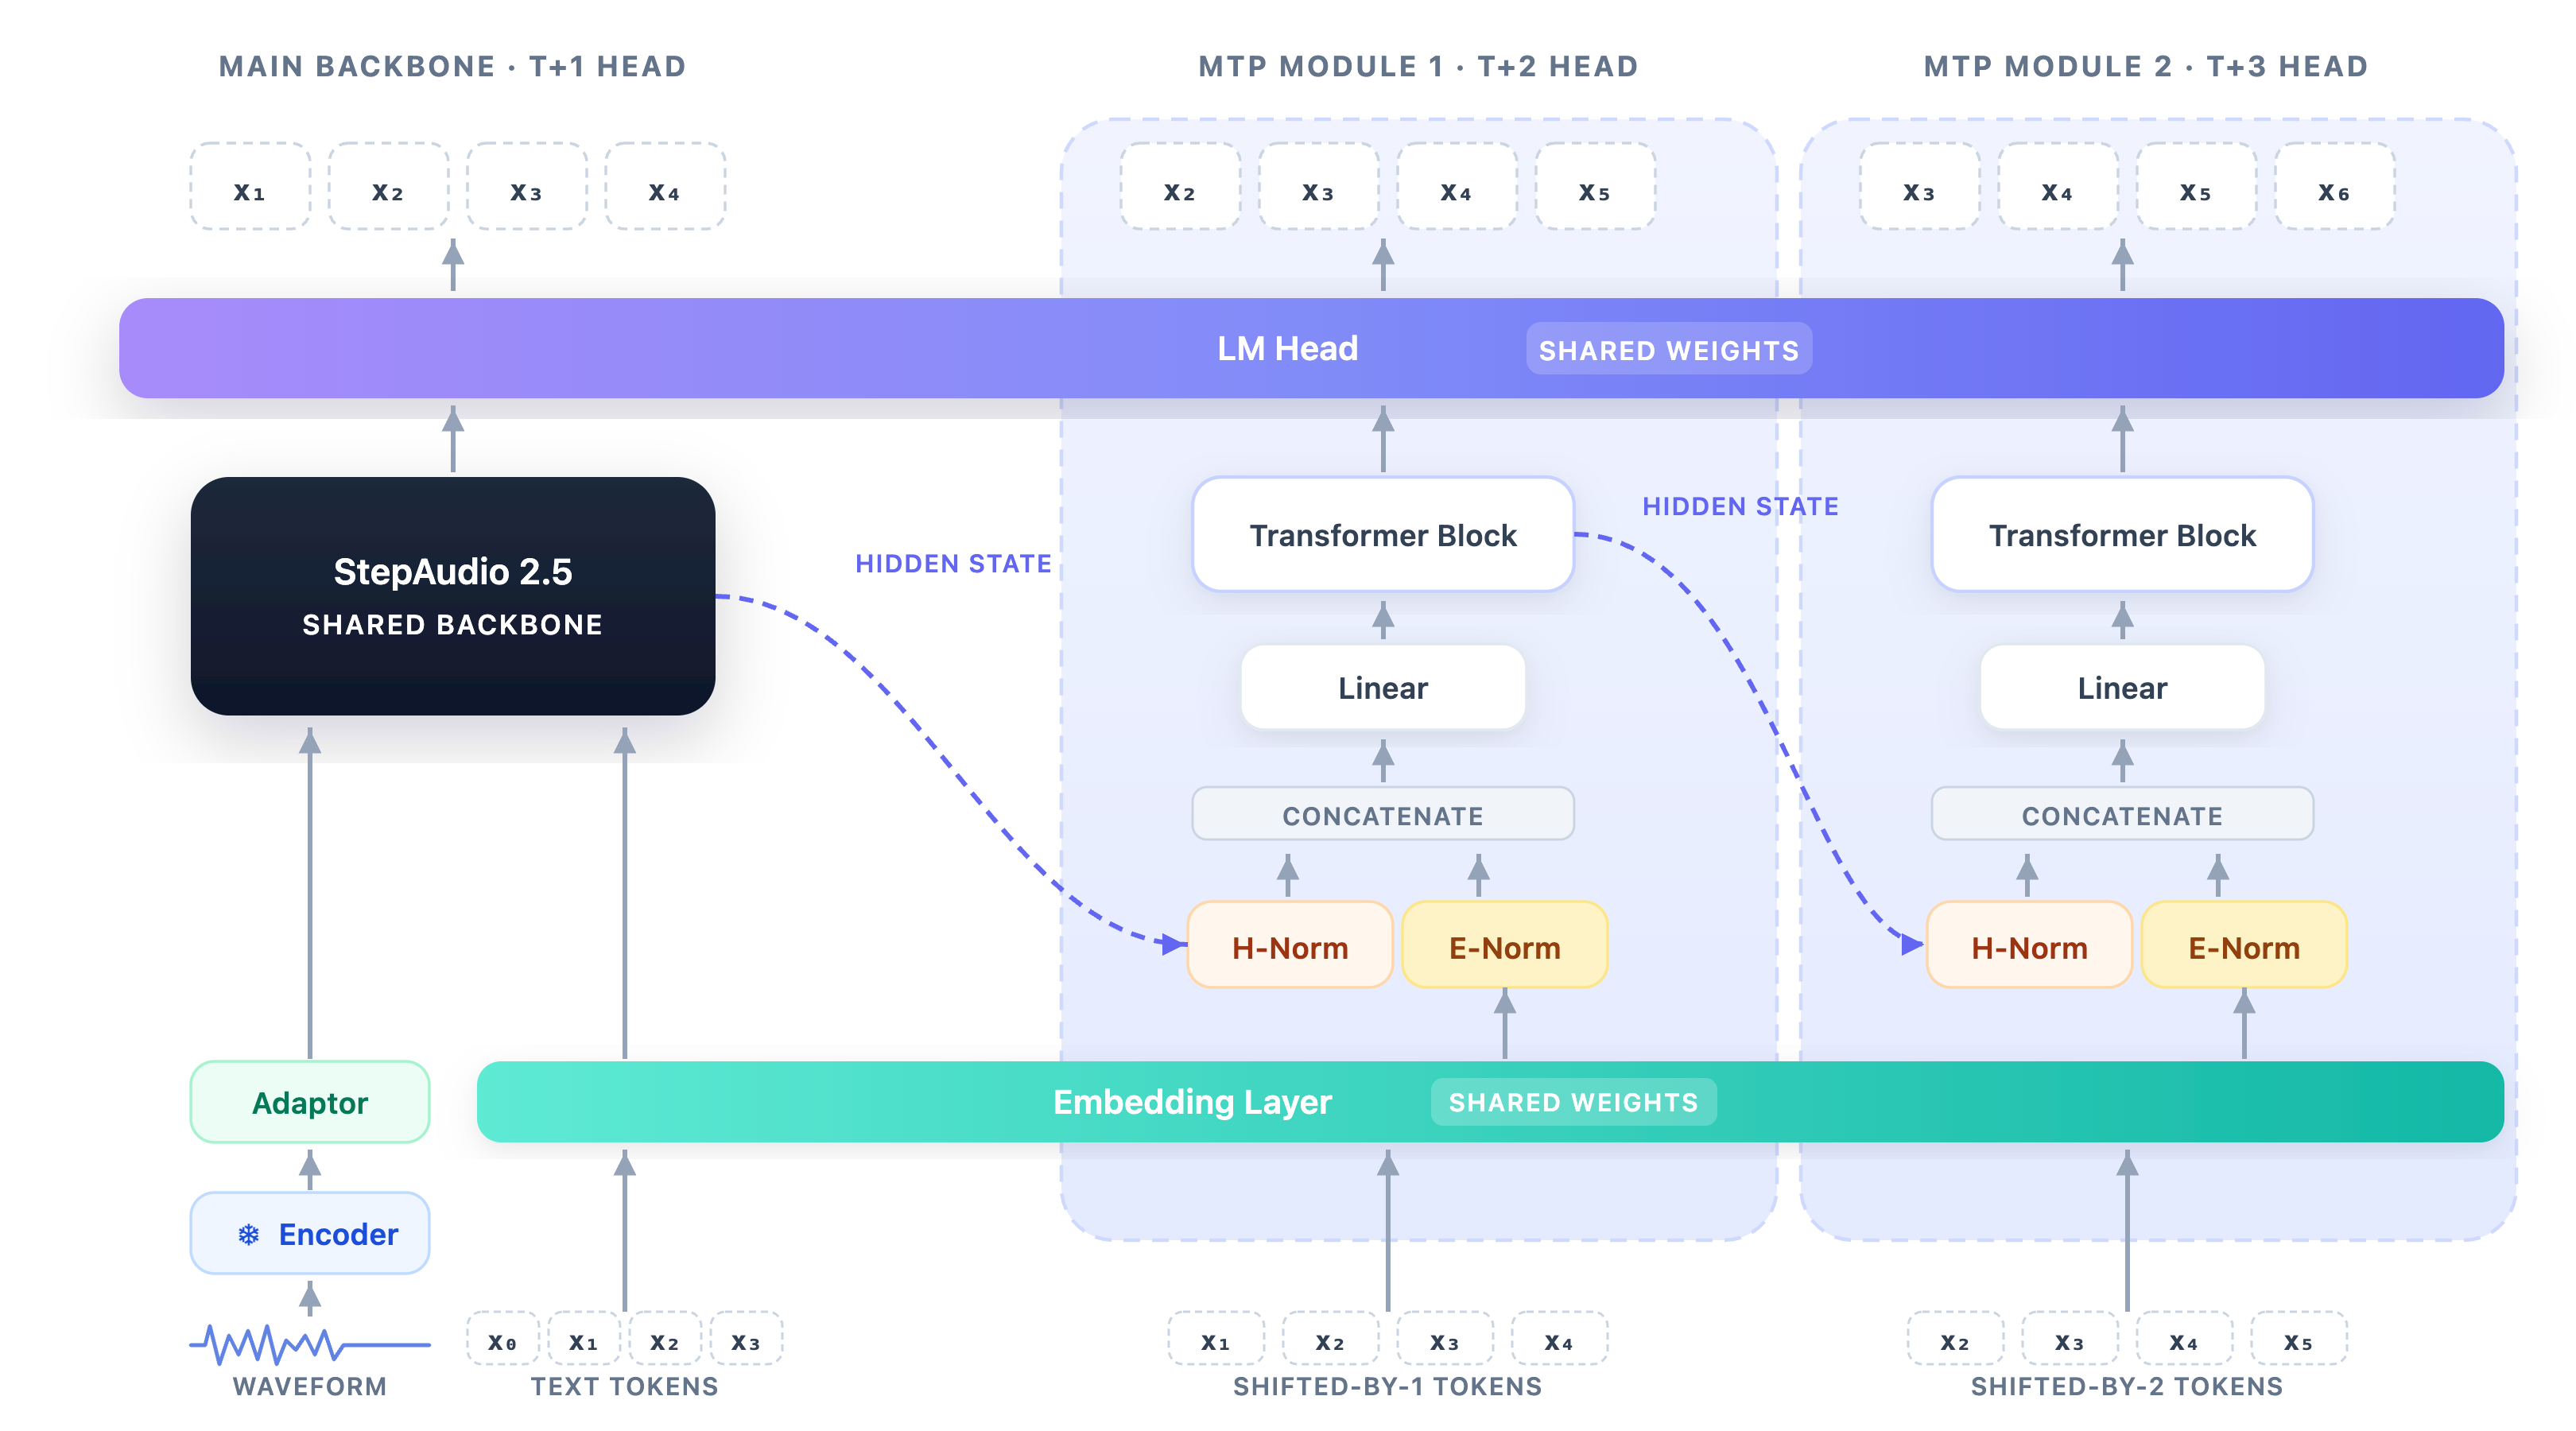
\includegraphics[width=\linewidth]{figures/stepaudio25-asr-mtp-architecture.png}
\caption{ASR architecture in StepAudio 2.5. The shared encoder-adaptor-decoder backbone is augmented with parallel future-token branches, making decoding substantially more efficient while preserving autoregressive verification.}
\label{fig:asr_architecture}
\end{figure}
% \textbf{Backbone architecture.} The backbone follows the standard encoder-adapter-decoder pattern for audio-language modeling. The audio encoder is a 0.6B Transformer initialized from Qwen3-Omni~\citep{xu2025qwen3omnitechnicalreport}. It remains frozen throughout training and applies 8x temporal downsampling to produce one acoustic embedding every 80 ms. These embeddings are projected by a linear adapter into the hidden space of the language decoder. The decoder is a proprietary 4B dense Transformer initialized from a pre-trained text LLM, supporting a native 32K context window. This large context budget, combined with the 80 ms acoustic embedding rate, allows StepAudio 2.5 ASR to process up to 30 minutes of audio in a single decoding session, eliminating the need for complex chunk-and-stitch pipelines.



% \textbf{Branch structure.} 
Each MTP block receives the hidden state from the previous branch and a shifted token embedding. The two inputs are normalized, concatenated, projected back to the decoder hidden size, and processed by a decoder-style Transformer block. All branches share the same embedding layer and vocabulary output head as the main decoder. % This structural alignment ensures that lookahead proposals remain linguistically consistent with the main autoregressive path.

\subsection{Training Pipeline}

\textbf{ASR SFT} Supervised fine-tuning first turns the model into a reliable autoregressive recognizer using both short-form and long-form data. Training examples are packed into a 32K-token sequence budget. SpecAugment-style time and frequency masking~\citep{park2019specaugment} is applied to the acoustic features. Throughout this stage, the audio encoder remains frozen, while the adapter and language decoder are optimized for 10K steps with a peak learning rate of $2\times10^{-5}$, a global batch size of 32, 100 warmup steps, and cosine decay to $1\times10^{-6}$.

\textbf{MTP Training} After the base recognizer has well converged, MTP is introduced as a lookahead proposal module through a staged optimization recipe: frozen-branch alignment and joint calibration. 

\begin{itemize}
    \item \textbf{Frozen-branch alignment.} Five MTP blocks are appended to the converged ASR decoder. The Transformer layer within each block is initialized from the last decoder layer to inherit a strong linguistic prior, while the branch-specific projections are newly initialized. In this stage, only the MTP blocks are optimized with a peak learning rate of $2\times10^{-4}$, while all other modules including the shared token embeddings and LM head remain frozen. % By decoupling the lookahead path from the recognition path, newly initialized branches are prevented from introducing noise into the established autoregressive behavior.
    \item \textbf{Joint calibration.} Once the branches have aligned with the ASR distribution, the adapter and LLM decoder are unfrozen for joint optimization with a lower learning rate of $2\times10^{-5}$. This stage reduces the residual mismatch between the backbone states and the lookahead branches, turning MTP into a calibrated proposal mechanism. % The optimization remains anchored to the transcription objective, ensuring that multi-token proposals stay tightly coupled with the acoustic evidence.
\end{itemize}

Both stages inherit the 32K sequence budget, 32 global batch size, and 10K-step training horizon.
During training, the main branch predicts the next token $x_{t+1}$ at position $t$, while the $h$-th MTP branch targets the future token $x_{t+1+h}$ for $h\in\{1,\ldots,H\}$. The branch weights are exponentially decayed to reflect the serial dependency of MTP:
\[
w_h = \frac{\alpha^{h-1}}{\sum_{j=1}^{H}\alpha^{j-1}}, \quad H=5, \quad \alpha=0.9.
\]
At each position $t$, the final objective combines the standard next-token loss with the weighted MTP losses:
\[
\mathcal{L}_t = \mathrm{CE}(p_t, x_{t+1}) + \sum_{h=1}^{H} w_h \mathrm{CE}(p_{t,h}, x_{t+1+h}),
\]
where $p_t$ and $p_{t,h}$ are the distributions from the main and auxiliary branches, respectively.


\subsection{Data}
\textbf{Short-form supervised data.} The short-form SFT set comprises approximately 100K hours of audio, integrating major public corpora with inhouse datasets. The mixture covers a wide spectrum of linguistic and acoustic variations, including Mandarin, English, and frequent code-switching utterances. To handle real-world complexity, the data also spans various vertical domains rich in professional terminologies, as well as challenging acoustic environments such as far-field recording and high-noise scenarios. Each sample in this set has a maximum duration of 30 seconds.

% \begin{figure}[tbp]
% \centering
% \resizebox{\textwidth}{!}{%
% \begin{tikzpicture}[
%     node distance=0.52cm and 0.62cm,
%     box/.style={draw, rounded corners, thick, align=center, minimum height=0.7cm, minimum width=1.8cm, fill=gray!8},
%     arrow/.style={-Latex, thick}
% ]
% \node[box] (crawl) {raw long\\recordings};
% \node[box, right=of crawl] (vad) {VAD\\segmentation};
% \node[box, right=of vad] (asr) {multi-system\\transcription};
% \node[box, right=of asr] (rover) {ROVER\\voting};
% \node[box, right=of rover] (filter) {quality\\filtering};
% \node[box, right=of filter] (concat) {session\\re-composition};
% \node[box, right=of concat] (repair) {LLM\\refinement};

% \draw[arrow] (crawl) -- (vad);
% \draw[arrow] (vad) -- (asr);
% \draw[arrow] (asr) -- (rover);
% \draw[arrow] (rover) -- (filter);
% \draw[arrow] (filter) -- (concat);
% \draw[arrow] (concat) -- (repair);
% \end{tikzpicture}%
% }
% \caption{Long-form ASR data construction pipeline. The process transitions from individual clip transcription to global session-level refinement to ensure both accuracy and consistency.}
% \label{fig:longdata}
% \end{figure}

\begin{figure}[tbp]
\centering
% \includegraphics[width=\linewidth]{figures/architecture.pdf}
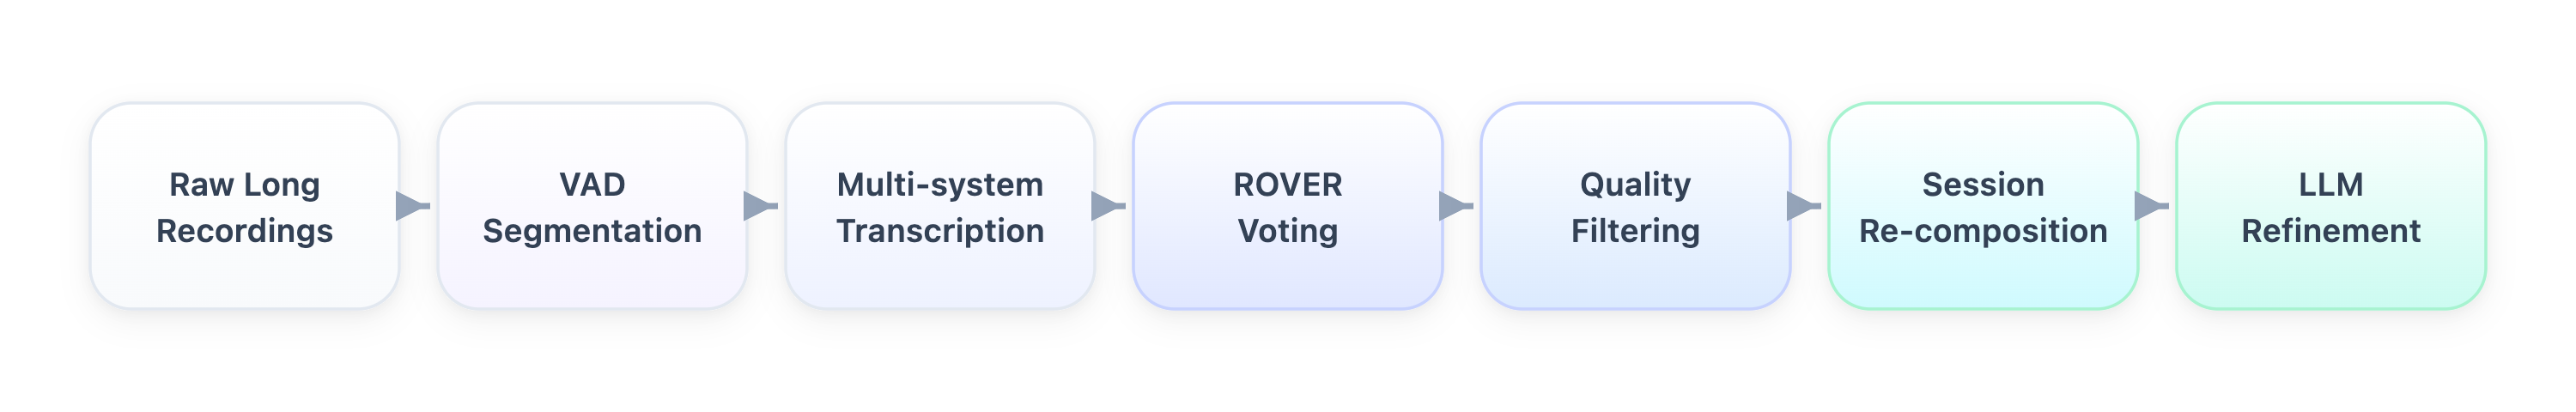
\includegraphics[width=\linewidth]{figures/stepaudio25-asr-data-pipeline.png}
\caption{Long-form ASR data construction pipeline. The process transitions from individual clip transcription to global session-level refinement to ensure both accuracy and consistency.}
\label{fig:longdata}
\end{figure}


\textbf{Long-form pseudo-labeled data.} While short-form data ensures utterance-level precision, long-duration recordings are essential for teaching the model to maintain contextual consistency. To support this capability, the training recipe curates a 50K-hour long-form dataset using a multi-system verification pipeline designed to provide reliable session-level supervision, as shown in Figure~\ref{fig:longdata}. Raw recordings are first segmented by Voice Activity Detection (VAD) into speech clips with a maximum duration of 30 seconds. Each clip is transcribed independently by three ASR systems to obtain multiple candidate hypotheses. To focus the subsequent fusion on genuine recognition errors, these hypotheses undergo surface-form normalization to unify formatting, casing, and punctuation. The normalized streams are then aligned and fused via Recognizer Output Voting Error Reduction (ROVER)~\citep{fiscus1997rover}, with voting performed at token level. Tokens are accepted only when supported by at least two systems, while non-consensus positions are marked as disagreements. The segment-level disagreement rate $\hat{e}$ serves as a proxy for label reliability:
\[
\hat{e}=\frac{\#\mathrm{disagreed\ positions}}{\#\mathrm{text\ units}}
\]
Clips with $\hat{e}>0.05$ are discarded to maintain high training signal fidelity. Passing neighbor segments are then concatenated into long-form training samples. Finally, an LLM-based refinement stage restores punctuation, performs inverse text normalization, and ensures cross-segment consistency by harmonizing recurring terminology and entities across the full session.

% Training examples are packed into a 32K-token sequence budget. SpecAugment-style time and frequency masking~\citep{park2019specaugment} is applied to the acoustic features. Throughout this stage, the audio encoder remains frozen, while the adapter and language decoder are optimized for 10K steps with a peak learning rate of $2\times10^{-5}$, a global batch size of 32, 100 warmup steps, and cosine decay to $1\times10^{-6}$.

\subsection{Evaluation}

The evaluation of StepAudio 2.5 ASR focuses on three primary objectives: recognition accuracy across diverse languages, native long-form transcription capability, and inference efficiency under production-scale serving. We compare the system against several competitive baselines, including VibeVoice-ASR~\citep{peng2026vibevoiceasrtechnicalreport}, FunASR-Nano~\citep{an2025funasrtechnicalreport}, Doubao-ASR-2603~\citep{bai2024seed} and Qwen3-ASR-1.7B~\citep{shi2026qwen3asrtechnicalreport}. To ensure a fair comparison, all models are deployed in a local environment using a single NVIDIA H800 GPU with single-concurrency serving, except for Doubao-ASR-2603, which is only accessible through the official API. For baseline models that do not natively support long-form audio like FunASR-Nano, VAD is used to segment recordings into clips with a maximum duration of 30 seconds. Recognition benchmarks draw on AISHELL-1~\citep{bu2017aishell}, AISHELL-2 (iOS test)~\citep{du2018aishell2}, WenetSpeech~\citep{zhang2022wenetspeech}, FLEURS~\citep{conneau2022fleurs}, LibriSpeech~\citep{panayotov2015librispeech}, Common Voice~\citep{ardila2020commonvoice}, VoxPopuli cleaned AA~\citep{artificialanalysis2026voxpopulicleaned}, and Earnings22 cleaned AA~\citep{artificialanalysis2026earnings22cleaned}. Long-form evaluation includes LibriSpeech long variants, Earnings22 cleaned AA, and WenetSpeech testnet long~\footnote{
WenetSpeech testnet long is constructed by merging adjacent WenetSpeech testnet segments into extended recordings. We release \url{https://github.com/lawlict/wenetspeech-testnet-long.git} for corpus generation.}.

% \subsubsection{Performance Benchmarks}

\textbf{Recognition performance.} Table~\ref{tab:asr_results} shows that StepAudio 2.5 ASR establishes a new performance frontier for LLM-based ASR. On Chinese benchmarks, the model improves the average CER to 2.97\%, with a notable reduction in error rate on AISHELL-1 to 0.71\% and a competitive 2.63\% on FLEURS zh. On English, the model reduces the average WER to 3.68\%, outperforming competitive baselines and showing particular strength on LibriSpeech clean (1.38\%) and VoxPopuli cleaned AA (2.76\%). Long-form transcription is where decoder context and linguistic depth matter simultaneously. The model reaches the best average long-form error rate of 3.70\%, representing a significant improvement over Qwen3-ASR-1.7B. The model is especially effective on the long LibriSpeech variants, where the native 32K context window allows it to maintain consistent recognition without the boundary errors typical of segmentation-based approaches.

We also compare StepAudio 2.5 ASR against the base ASR model after SFT but before MTP training. Across Chinese, English, and long-form benchmarks, the addition of MTP-5 leaves recognition accuracy essentially unchanged, with average fluctuations within 0.06 absolute points. This stability is the result of the staged training recipe and the autoregressive verification process, which ensures that the final transcript is always determined by the verified path.


% \begin{figure}[tbp]
% \centering
% \includegraphics[width=\linewidth]{figures/asr_benchmark_chart.pdf}
% \caption{ASR performance overview in StepAudio 2.5. Lower is better. The figure summarizes the unusual combination of strong recognition quality and high-throughput decoding.}
% \label{fig:asr_benchmark}
% \end{figure}

\begin{table}[tbp]
\centering
\small
\setlength{\tabcolsep}{3.2pt}
\caption{ASR results on Chinese, English, and long-form benchmarks (Error Rate, \%). Lower is better. The second-best results are underlined.}
\label{tab:asr_results}
\begin{adjustbox}{max width=\textwidth}
\begin{tabular}{llcccccc>{\color{gray}\arraybackslash}c}
\toprule
Category & Test set & VibeVoice-ASR & FunASR-Nano & Doubao-ASR-2603 & Qwen3-ASR-1.7B & StepAudio 2.5 ASR & \textcolor{gray}{\makecell{StepAudio 2.5 ASR\\w/o MTP training}} \\
\midrule
\multirow{6}{*}{Chinese}
& AISHELL-1 & 5.19 & 1.88 & 2.07 & \underline{1.49} & \textbf{0.71} & \textcolor{gray}{0.79} \\
& AISHELL-2 ios & 5.10 & 2.61 & 2.70 & \underline{2.50} & \textbf{2.29} & \textcolor{gray}{2.30} \\
& WenetSpeech testnet & 14.79 & 5.30 & \textbf{4.03} & \underline{4.44} & 4.54 & \textcolor{gray}{4.57} \\
& WenetSpeech testmeeting & 17.09 & 5.31 & 5.09 & \textbf{4.66} & \underline{4.70} & \textcolor{gray}{4.73} \\
& FLEURS zh & 8.77 & 3.19 & 2.83 & \underline{2.74} & \textbf{2.63} & \textcolor{gray}{2.63} \\
\cmidrule(lr){2-8}
& Average & 10.19 & 3.66 & 3.34 & \underline{3.17} & \textbf{2.97} & \textcolor{gray}{3.00} \\
\midrule
\multirow{6}{*}{English}
& LibriSpeech clean & 2.30 & 1.80 & 2.94 & \underline{1.69} & \textbf{1.38} & \textcolor{gray}{1.40} \\
& LibriSpeech other & 5.79 & 4.43 & 5.98 & \underline{3.57} & 3.16 & \textcolor{gray}{3.14} \\
& Common Voice v11 en & 20.03 & 11.05 & 14.06 & \textbf{7.50} & \underline{7.57} & \textcolor{gray}{7.62} \\
& FLEURS en & 5.20 & 4.96 & 6.74 & \textbf{3.23} & \underline{3.55} & \textcolor{gray}{3.74} \\
& VoxPopuli cleaned AA & \textbf{2.38} & 3.97 & 3.61 & 3.28 & \underline{2.76} & \textcolor{gray}{3.23} \\
\cmidrule(lr){2-8}
& Average & 7.14 & 5.24 & 6.67 & \underline{3.85} & \textbf{3.68} & \textcolor{gray}{3.83} \\
\midrule
\multirow{5}{*}{Long-form}
& LibriSpeech clean long & \underline{1.66} & 2.34 & 2.81 & 1.95 & \textbf{1.27} & \textcolor{gray}{1.27} \\
& LibriSpeech other long & 3.48 & 4.89 & 5.59 & \underline{3.81} & 2.90 & \textcolor{gray}{2.81} \\
& WenetSpeech testnet long & 8.73 & 4.74 & \textbf{3.72} & 4.15 & \underline{4.09} & \textcolor{gray}{4.09} \\
& Earnings22 cleaned AA & \textbf{5.62} & 10.38 & 12.33 & 6.90 & \underline{6.52} & \textcolor{gray}{6.34} \\
\cmidrule(lr){2-8}
& Average & 4.87 & 5.59 & 6.11 & 4.20 & \underline{3.70} & \textcolor{gray}{3.63} \\
\bottomrule
\end{tabular}
\end{adjustbox}
\end{table}

\textbf{Decoding efficiency.} Table~\ref{tab:rtf} evaluates the deployment objective directly. The Real-Time Factor is measured on 100 clips of 30 seconds each. StepAudio 2.5 ASR reaches an exceptionally low RTF of 0.0053, faster than the Qwen3-ASR-1.7B baseline despite using a larger decoder. It is also substantially faster than VibeVoice-ASR, FunASR-Nano, and Doubao-ASR-2603 under the same serving setup. This is the key systems consequence of MTP for ASR: decoder scale no longer translates linearly into token-by-token latency, because most steps emit several verified transcript tokens.

\begin{table}[htb]
\centering
\small
\caption{RTF comparison.}
\label{tab:rtf}
\begin{tabular}{lccccc}
\toprule
Model & VibeVoice-ASR & FunASR-Nano & Doubao-ASR-2603 & Qwen3-ASR-1.7B & StepAudio 2.5 ASR \\
\midrule
RTF & 0.1039 & 0.0591 & 0.0640 & 0.0094 & \textbf{0.0053} \\
\bottomrule
\end{tabular}
\end{table}

\textbf{MTP acceptance behavior.} Experiments evaluate the strict per-position acceptance rate on the WenetSpeech meeting set~\citep{zhang2022wenetspeech}. To determine the optimal lookahead horizon, three configurations are compared: MTP-3, MTP-5, and MTP-7. Results in Table~\ref{tab:acceptance} reveal two primary trends. First, the acceptance rates of earlier positions are nearly invariant to the total number of branches, indicating that each MTP head learns a stable, independent prediction task. Second, starting from the second position, the acceptance rate decays at a consistent factor of approximately $0.9$ per branch. While increasing branches from three to five yields a substantial 39\% gain in average accepted length, the additional step to MTP-7 provides a more modest improvement about 22\%. This diminishing return is driven by the high failure rates of the sixth and seventh positions, which frequently trigger KV cache rollbacks and interrupt the decoding stream, and finally offset the marginal utility of a longer lookahead. Consequently, MTP-5 represents a deliberate choice for the optimal efficiency-complexity trade-off.

\begin{table}[htb]
\centering
\small
\setlength{\tabcolsep}{8pt}
\caption{Strict per-position MTP acceptance rate and average accepted length.}
\label{tab:acceptance}
\begin{adjustbox}{max width=\textwidth}
\begin{tabular}{lccccccc|c}
\toprule
Config & 1st & 2nd & 3rd & 4th & 5th & 6th & 7th & Avg. Length \\
\midrule
MTP-3 & 0.96 & 0.88 & 0.80 & -- & -- & -- & -- & 3.6 / 4 \\
MTP-5 & 0.95 & 0.88 & 0.80 & 0.71 & 0.64 & -- & -- & 5.0 / 6 \\
MTP-7 & 0.96 & 0.88 & 0.80 & 0.72 & 0.65 & 0.59 & 0.53 & 6.1 / 8 \\
\bottomrule
\end{tabular}
\end{adjustbox}
\end{table}


\textbf{Insight.} The ASR branch suggests a useful general lesson for multimodal systems: grounded generation tasks can sometimes be accelerated more aggressively than free-form text generation, precisely because the external modality reduces semantic branching. In other words, grounding is not only a source of information; it is also a source of algorithmic structure.
